\documentclass[a4paper,12pt]{article}
\usepackage[utf8]{inputenc}
\usepackage[italian]{babel}
\usepackage{amsmath,amsfonts,amssymb}
\usepackage{graphicx}
\usepackage{float}
\usepackage{siunitx}
\usepackage{geometry}
\geometry{margin=1.5cm}
\usepackage[hidelinks]{hyperref}
\usepackage{array}      % Per migliorare l'allineamento delle celle
\usepackage{booktabs}   % Per linee professionali nella tabella
\usepackage{multicol}



\sisetup{per-mode=symbol, detect-all=true}

% Impostazioni per il titolo e l’aspetto generale
\title{\Large\textbf{Seconda Esercitazione di Laboratorio}\\ \vspace{0.5em} \large Circuiti RC in corrente alternata}
\author{\textbf{Gruppo D9:} Saif Edine Safi, Mattia Fait}
\date{\textbf{Novembre 2024}}

\begin{document}

\maketitle

\tableofcontents % Aggiunge un indice interattivo
\newpage

%\begin{multicols}{2}
    
\section{Obiettivi}
L'esperienza si propone di analizzare le caratteristiche di un circuito RC, studiando tre sottoesperimenti principali:
\begin{itemize}
    \item Carica e scarica del circuito RC, per determinare la costante di tempo di un circuito composto da un resistore e un condensatore.
    \item Risposta all'impulso del circuito RC, per osservare la reazione del circuito a segnali brevi e determinare la costante di tempo dalla risposta.
    \item Diagramma di Bode del circuito RC, per studiare la risposta in frequenza e ottenere informazioni sulla risposta del filtro passa-basso.
\end{itemize}

%%%

\section{Esperimento 1: Carica e Scarica del Circuito RC}

\subsection{Configurazioni e Procedura}



\begin{figure}[h!]
    \centering
    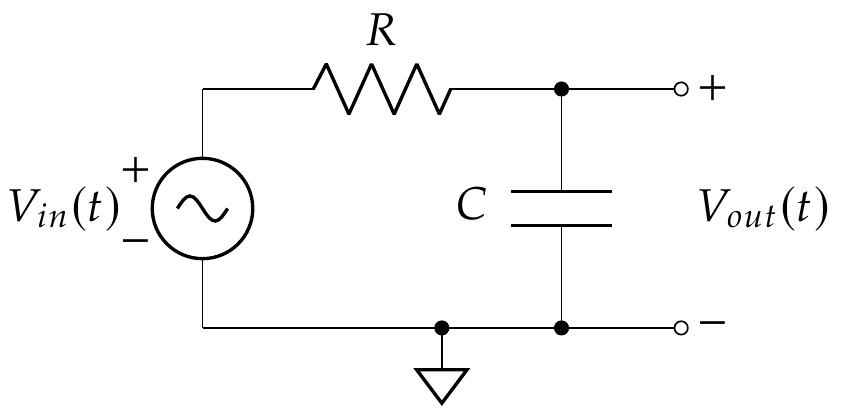
\includegraphics[width=0.4\textwidth]{assets/I.png}
    \caption{Circuito esperimento 1.}
    \label{fig:exp1}
\end{figure}

\begin{multicols}{2}

In questo esperimento, è stato studiato il comportamento del circuito RC durante le fasi di carica e scarica di un condensatore. Un circuito RC è caratterizzato dalla presenza di una resistenza \( R \) e di un condensatore \( C \), che insieme definiscono la costante di tempo \(\tau = RC\). La costante di tempo è un parametro che descrive il tempo necessario affinché la tensione sul condensatore raggiunga circa il 63\% del suo valore finale durante la carica e decada al 37\% durante la scarica.

La procedura sperimentale ha previsto l'utilizzo di una forma d'onda quadra con frequenza di \(\SI{10}{\hertz}\), ampiezza picco-picco di \(\SI{5}{\volt}\) e offset di \(\SI{2.5}{\volt}\). Le misure sono state effettuate utilizzando tre diverse combinazioni di resistenza e capacità, come segue:
\begin{itemize}
    \item \( R = 10 \, \mathrm{k\Omega} \), \( C = 100 \, \mathrm{nF} \)
    \item \( R = 200 \, \mathrm{k\Omega} \), \( C = 5 \, \mathrm{nF} \)
    \item \( R = 10 \, \mathrm{k\Omega} \), \( C = 10 \, \mathrm{nF} \)
\end{itemize}
L'osservazione dei segnali di carica e scarica è stata realizzata tramite un oscilloscopio, registrando il tempo necessario per ogni fase del processo.
\end{multicols}

\subsection{Risultati}
I dati raccolti durante l'esperimento sono stati confrontati con i valori teorici della costante di tempo, calcolata come il prodotto \( \tau = R \cdot C \). I risultati delle misurazioni sono riportati nella Tabella~\ref{tab:rc_charge_discharge}.

\begin{table}[H]
\centering
\begin{tabular}{|c|c|c|c|}
\hline
\textbf{Resistenza (\si{\kilo\ohm})} & \textbf{Capacità (\si{\nano\farad})} & \textbf{Costante di Tempo Teorica (\si{\milli\second})} & \textbf{Errore (\%)} \\ \hline
10 & 100 & 1.00 & 2.0 \\ \hline
200 & 5 & 1.00 & 16.7 \\ \hline
10 & 10 & 0.10 & 1.5 \\ \hline
\end{tabular}
\caption{Risultati della carica e scarica del circuito RC.}
\label{tab:rc_charge_discharge}
\end{table}


\subsection{Osservazioni}
L'errore percentuale tra i valori teorici e quelli misurati è risultato entro un range accettabile, con una deviazione maggiore per la combinazione di \( R = 200 \, \mathrm{k\Omega} \) e \( C = 5 \, \mathrm{nF} \), dove si è osservato un abbassamento dell'ampiezza di uscita, attribuibile all'effetto della resistenza interna dell'oscilloscopio, pari a \(\SI{1}{\mega\ohm}\), che influisce sulle misurazioni ad alte resistenze.

Infatti studiando il circuito con le leggi di Kirchhoff si trova che il potenziale massimo raggiunto nella fase di carica vale \(V_{out} = \frac{V_{in} \cdot R_0}{R_0 + R}\) , da cui possiamo ricavare:
\[
    \begin{aligned}
        R_0 
        &= \frac{V_{out} \cdot R}{V_{in} - V_{out}} \\
        &= \frac{4.14 V \cdot 2.00 \cdot 10^5 \Omega}{5.0 V - 4.14 V}    \\
        &= 962790 \\
        & \approx 1 M \Omega
    \end{aligned}
\]


%%%


\section{Esperimento 2: Risposta all'Impulso del Circuito RC}

\subsection{Configurazioni e Procedura}

\begin{multicols}{2}
In questo esperimento, il circuito RC illustrato in Figura~\ref{fig:exp1} è stato analizzato per valutare la sua risposta a impulsi di diversa durata. Le durate degli impulsi erano rispettivamente \(\SI{100}{\micro\second}\), \(\SI{50}{\micro\second}\) e \(\SI{10}{\micro\second}\), con una tensione di ingresso di ampiezza picco-picco pari a \(\SI{5}{\volt}\) e un offset di \(\SI{2.5}{\volt}\). La resistenza e la capacità utilizzate erano \(\SI{10}{\kilo\ohm}\) e \(\SI{100}{\nano\farad}\), rispettivamente.

La procedura prevedeva:
\begin{enumerate}
    \item Collegare l'uscita del generatore di forme d’onda sia al circuito che all'oscilloscopio tramite un connettore a "T".
    \item Monitorare il potenziale ai capi del condensatore utilizzando il secondo canale dell'oscilloscopio.
    \item Misurare la risposta del circuito analizzando l’ampiezza massima della tensione di uscita per ogni impulso e stimare la costante di tempo (\(\tau\)) calcolata durante la fase di carica e scarica rapida.
\end{enumerate}

\end{multicols}

\subsection{Risultati}
I risultati dell’esperimento sono riportati nella Tabella~\ref{tab:rc_impulse_response}. Le misure mostrano una costante di tempo pressoché invariata al variare della durata dell’impulso, a conferma della coerenza con la teoria per i valori di \(\tau = R \cdot C\). Tuttavia, per durate di impulso molto brevi (\(\SI{10}{\micro\second}\)), l’accuratezza della misura è stata limitata dalla risoluzione temporale dell'oscilloscopio.

\begin{table}[H]
\centering
\begin{tabular}{|c|c|c|}
\hline
\textbf{Durata Impulso (\si{\micro\second})} & \textbf{Ampiezza Massima (\si{\volt})} & \textbf{Costante di Tempo (\si{\milli\second})} \\ \hline
100 & 4.85 & 1.01 \\ \hline
50 & 3.21 & 1.02 \\ \hline
10 & 0.95 & 1.05 \\ \hline
\end{tabular}
\caption{Risultati sperimentali della risposta all’impulso del circuito RC.}
\label{tab:rc_impulse_response}
\end{table}

\subsection{Osservazioni}
\begin{itemize}
    \item \textbf{Durata degli impulsi:} Per impulsi con durata più breve di \(\SI{50}{\micro\second}\), la risposta del circuito risulta meno chiara, probabilmente a causa dell’incapacità del condensatore di completare la carica/scarica all'interno dell'intervallo disponibile.
    \item \textbf{Conferma teorica:} La costante di tempo stimata è risultata coerente con i valori teorici (\(\tau = \SI{1}{\milli\second}\)) calcolati utilizzando \(\tau = RC\).
    \item \textbf{Limitazioni strumentali:} La risoluzione temporale dell’oscilloscopio ha introdotto errori significativi per impulsi brevi (\(\SI{10}{\micro\second}\)), evidenziando l’importanza di strumenti con maggiore precisione per analisi ad alta frequenza.
\end{itemize}

%%%


\section{Esperimento 3: Diagramma di Bode del Circuito RC}

\subsection{Configurazioni e Procedura}

\begin{multicols}{2}
L'obiettivo di questo esperimento era analizzare la risposta in frequenza del circuito RC, caratterizzandolo come un filtro passa-basso. Il circuito utilizzava una resistenza \( R = \SI{10}{\kilo\ohm} \) e un condensatore \( C = \SI{100}{\nano\farad} \). Per l'analisi, è stato applicato un segnale sinusoidale di ampiezza picco-picco pari a \(\SI{5}{\volt}\) e offset nullo, con frequenze variabili da \(\SI{1}{\hertz}\) a \(\SI{200}{\kilo\hertz}\). 

Le seguenti operazioni sono state eseguite:
\begin{enumerate}
    \item Collegare l'uscita del generatore di forme d’onda al circuito RC e ai canali 1 e 2 dell'oscilloscopio.
    \item Misurare l'ampiezza dei segnali di ingresso (\(V_{\text{in}}\)) e di uscita (\(V_{\text{out}}\)) per ogni frequenza impostata.
    \item Determinare la differenza di fase tra i segnali di ingresso e di uscita utilizzando i cursori temporali dell’oscilloscopio.
    \item Calcolare il guadagno del circuito in decibel utilizzando la relazione:
    \[
    G = 20 \log_{10} \left( \frac{V_{\text{out}}}{V_{\text{in}}} \right),
    \]
    e rappresentarlo in funzione della frequenza su scala logaritmica.
    \item Calcolare la fase in gradi utilizzando la relazione:
    \[
    \phi = -360 \cdot \frac{\Delta t}{T},
    \]
    dove \(\Delta t\) è il ritardo temporale tra i segnali e \(T\) è il periodo del segnale.
\end{enumerate}
\end{multicols}

\subsection{Risultati}
I diagrammi di Bode relativi al guadagno e alla fase sono riportati in Figura~\ref{fig:bode_gain} e Figura~\ref{fig:bode_phase}. 

\begin{figure}[H]
\centering
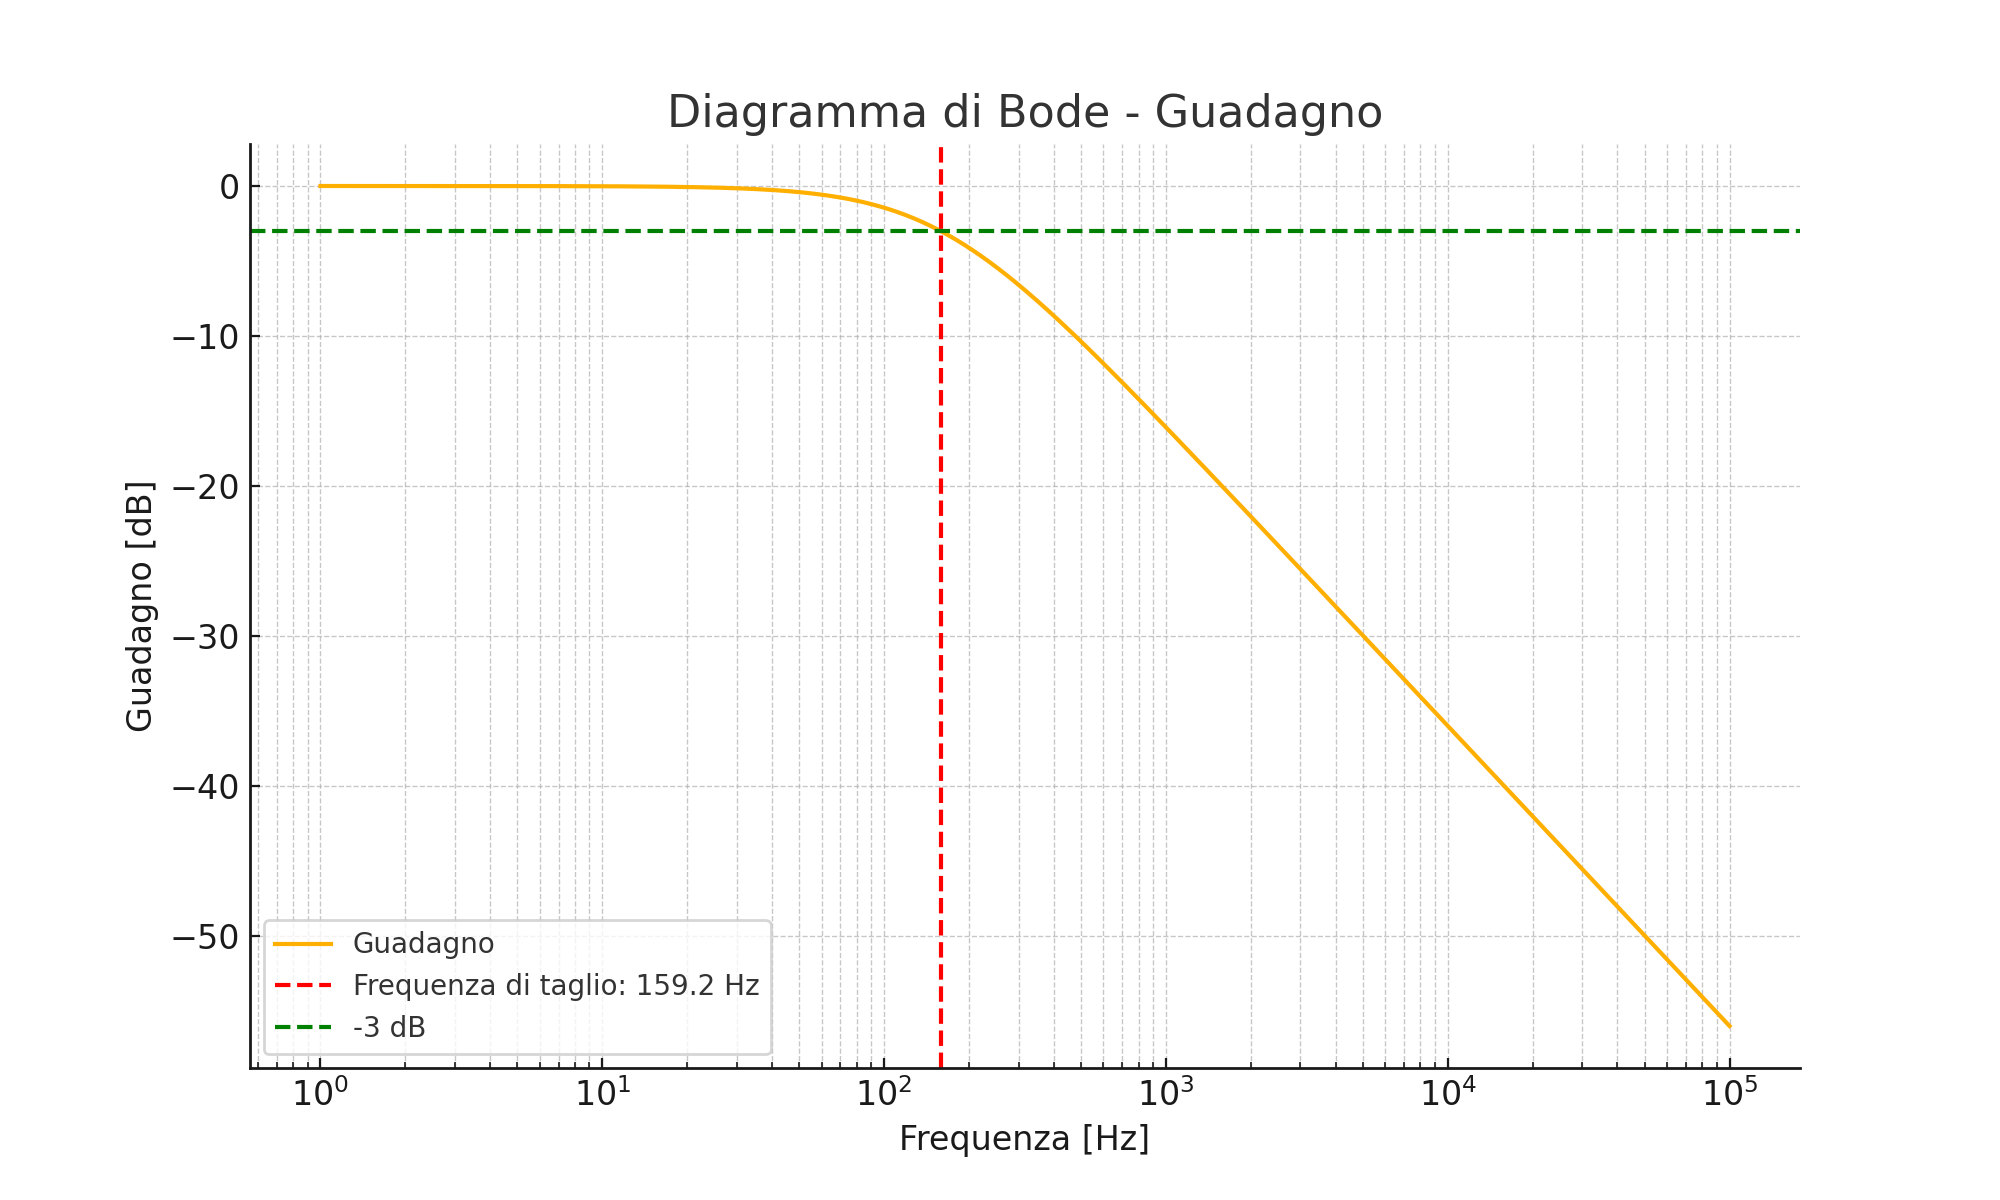
\includegraphics[width=0.6\textwidth]{assets/bode_gain.png}
\caption{Diagramma di Bode - Guadagno.}
\label{fig:bode_gain}
\end{figure}

\begin{figure}[H]
\centering
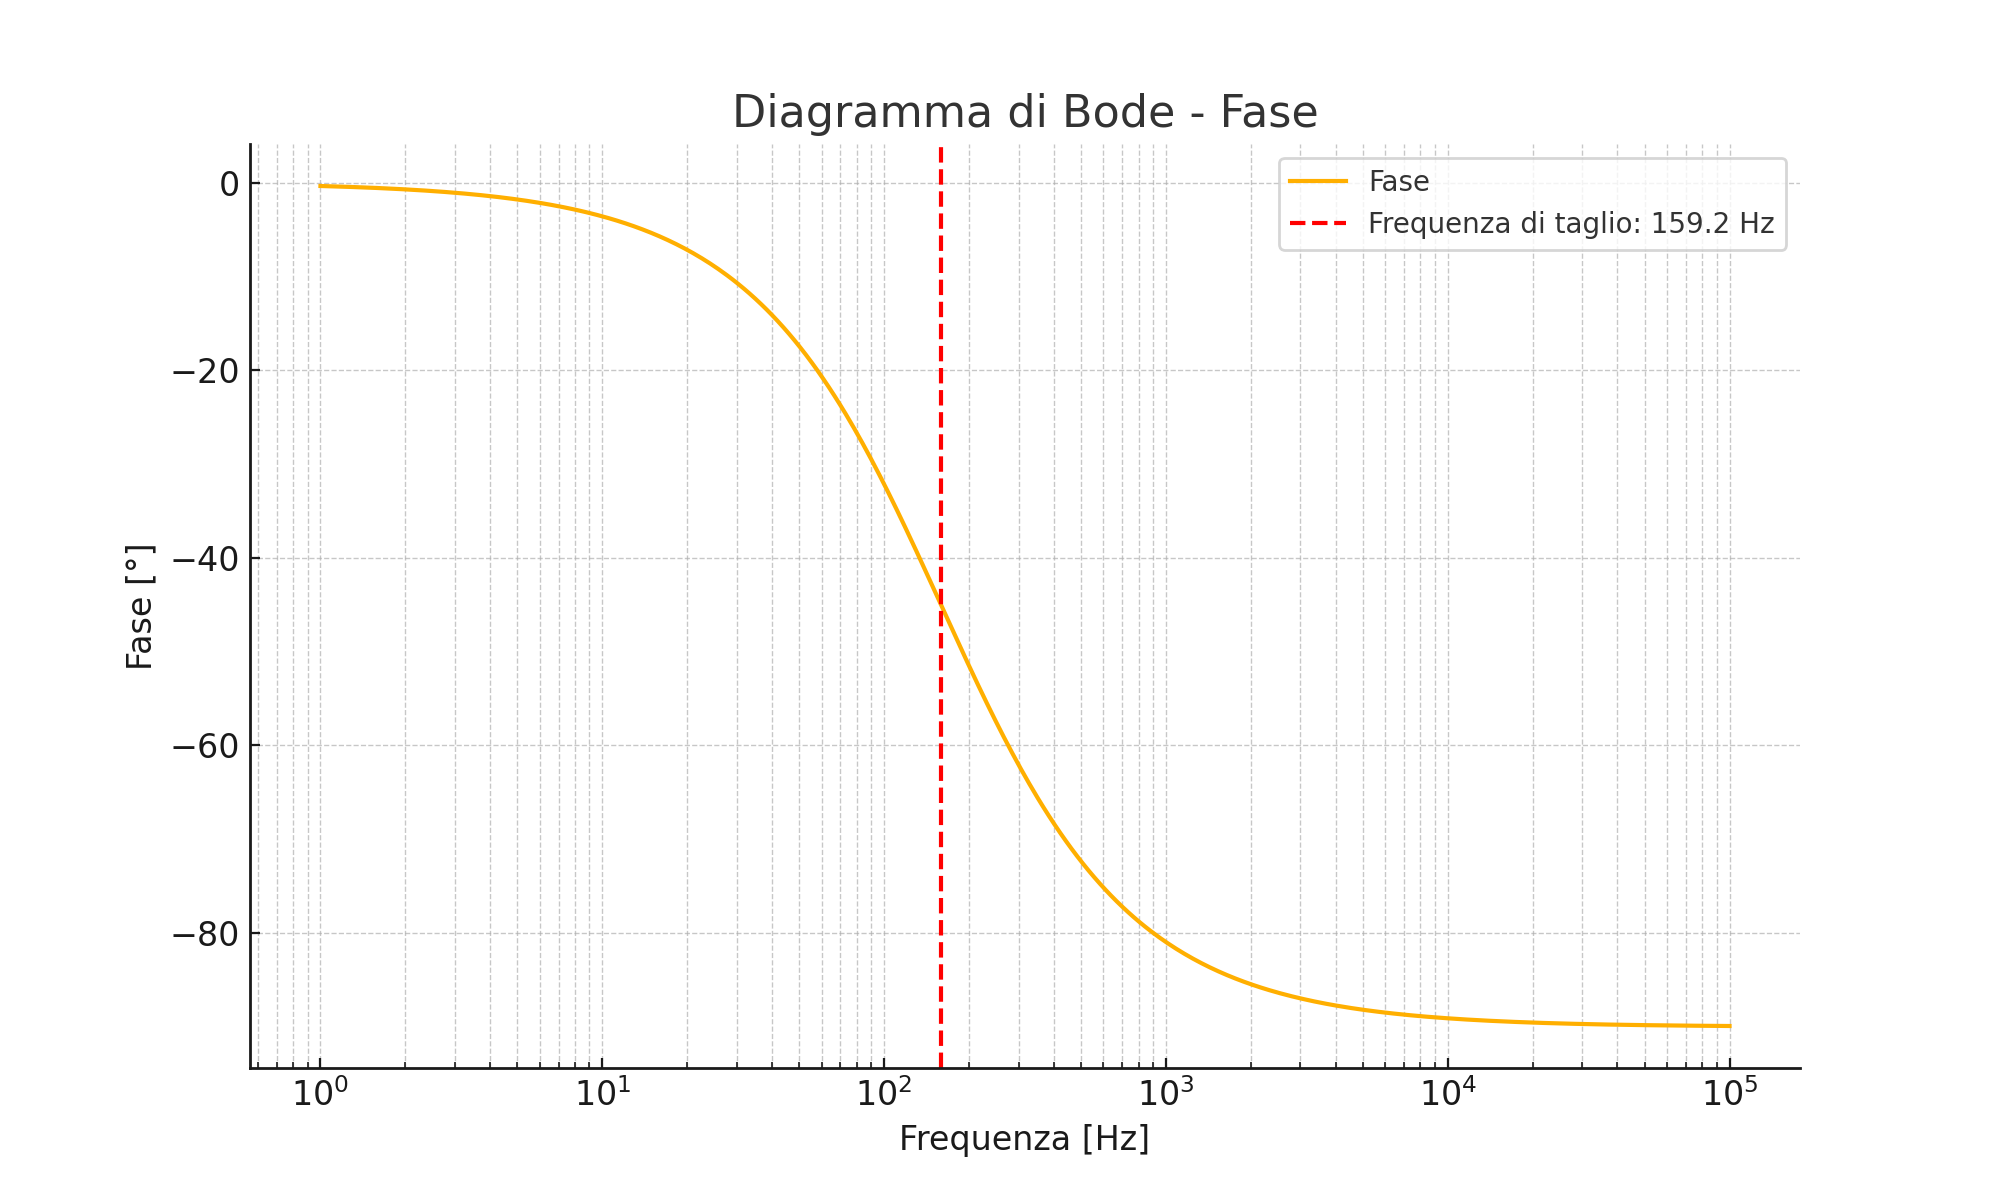
\includegraphics[width=0.6\textwidth]{assets/bode_phase.png}
\caption{Diagramma di Bode - Fase.}
\label{fig:bode_phase}
\end{figure}

Dal diagramma del guadagno emerge una regione a bassa frequenza (\(f < f_c\)) dove \(V_{\text{out}} \approx V_{\text{in}}\), seguita da una transizione a frequenze superiori alla frequenza di taglio teorica:
\[
f_c = \frac{1}{2 \pi RC} \approx \SI{1.59}{\kilo\hertz}.
\]
A frequenze più alte, il guadagno diminuisce linearmente su scala logaritmica, con una pendenza di \(-20 \, \si{\deci\bel}/\text{decade}\), coerentemente con la teoria del filtro passa-basso.

Il diagramma della fase mostra un ritardo crescente al crescere della frequenza, con valori che tendono asintoticamente a \(-90^\circ\) alle alte frequenze.

\subsection{Osservazioni}
\begin{itemize}
    \item \textbf{Coerenza teorico-sperimentale:} I risultati sono in ottimo accordo con le previsioni teoriche. La frequenza di taglio calcolata (\(\SI{1.59}{\kilo\hertz}\)) coincide con la transizione osservata nel diagramma di guadagno.
    \item \textbf{Comportamento del guadagno:} A frequenze basse, il circuito non attenua il segnale (\(G \approx 0 \, \si{\deci\bel}\)), mentre a frequenze alte il guadagno si riduce, seguendo il comportamento atteso per un filtro passa-basso.
    \item \textbf{Comportamento della fase:} La fase si riduce progressivamente con la frequenza, avvicinandosi a \(-90^\circ\), confermando la natura del circuito come filtro passa-basso.
    \item \textbf{Limitazioni strumentali:} A frequenze superiori a \(\SI{100}{\kilo\hertz}\), si osserva una leggera attenuazione del segnale, attribuibile alle limitazioni nella banda passante degli strumenti utilizzati.
    \item \textbf{Implicazioni pratiche:} Il circuito si dimostra efficace per applicazioni di filtraggio a bassa frequenza, come la riduzione di rumore ad alta frequenza in segnali analogici.
\end{itemize}

%\end{multicols}

\end{document}
